\chapter{Experimento Simulado}
\label{Capitulo_3}
\label{ExperimentoSimulado}
Antes de plantear un experimento real, decidimos probar nuestro sistema en un caso experimental. Para eso, se decidió usar \acs{ns3} (\acl{ns3}). \acs{ns3} es un simulador de redes que permite no solo emular protocolos de enrutamiento como \acs{odv} (\acl{odv}) sino también aplicarle movilidad a los nodos y utilizar distintos modelos de \textit{Path Loss}.
Para este experimento simulado, se decidió configurar una red \textit{Ad Hoc} entre todos los nodos. Y se usó un modelo de propagación ideal: el \textbf{ns3::FriisPropagationLossModel}.
Uno de los nodos, nuestro \textbf{Objetivo}, se configuró como el nodo transmisor. Este emite mensajes constantemente de tipo \textit{broadcast} que, al estar conectados en una red \textit{ad hoc}, todos reciben.
Cada nodo tiene un script que, al recibir un mensaje de \textit{broadcast} del nodo \textbf{Objetivo}, guarda la ubicación real de este y el \textbf{RSSI} con el que se recibió el paquete.
Mientras esto ocurre, usando un modelo de movilidad, se le aplica un recorrido al nodo \textbf{Objetivo}. Mientras tanto, los otros nodos, que hacen las veces de \textit{Sniffer}, permanecen quietos durante todo el experimento. Al finalizar la simulación, se recopilan los datos en un archivo \textit{.csv} para luego ser analizados por herramientas propias.
\section{Perfilado}
\subsection{Implementación}
\begin{figure}[!htb]
\centering
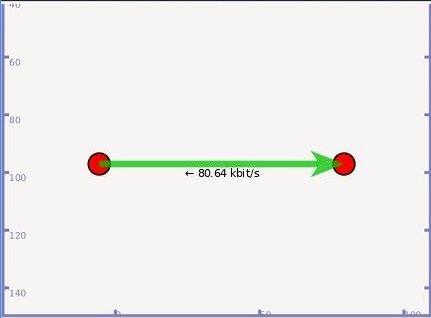
\includegraphics[width=0.5\textwidth]{Figuras/profiling/simulation/profiling_pyvis_going_away2.jpg}
\captionsetup{margin=2cm}
\caption[Visualización de la simulacion de NS3. El nodo objetivo se aleja del nodo Sniffer.]{Visualización de la simulación de \acs{ns3}. El nodo objetivo se aleja de uno de los nodos \textit{Sniffer}.}
\label{fig:simulated-ns3-profiling}
\end{figure}
En el caso del experimento de perfilado simulado, se utilizó un solo nodo \textit{Sniffer} que recibe paquetes de un nodo \textit{Objetivo} a medida que este se aleja. El resultado de la simulación es un archivo \textit{CSV} compuesto por filas (\textbf{distancia}, \textbf{rssi}). Finalmente, tomamos estos datos de \acs{rssi}, más los datos reales de distancia (calculados en la misma simulación) y realizamos un ajuste de curva hasta encontrar los valores de \textbf{N} y \textbf{A}. Estos nos servirán más adelante para predecir la distancia de dicho nodo en base a su \acs{rssi}.
El código para este experimento se encuentra en el siguiente archivo \href{https://github.com/agusalex/ns3-rssi-trilateration/blob/main/src/1DDistanceProfiling.cc}{\textbf{1DDistanceProfiling.cc}}.
Finalmente, se graficó la señal y la curva usando \textit{pyplot}.
\subsection{Experimento}
\begin{table}[!htb]
\centering
\begin{tabular}{|c|c|}
\hline
distance & rssi \\
\hline
10 & -52.55195 \\
11 & -54.77925 \\
12 & -56.68085 \\
13 & -58.339575 \\
14 & -59.810625 \\
15 & -61.132175 \\
16 & -62.33185 \\
17 & -63.43025 \\
18 & -64.443175 \\
19 & -65.383025 \\
20 & -66.2595 \\
21 & -67.080725 \\
22 & -67.85325 \\
23 & -68.5825 \\
24 & -69.273075 \\
25 & -69.928875 \\
\hline
\end{tabular}
\caption{Extracto de captura simulada de perfilado (capture.csv)}
\label{table:1}
\end{table}
Para poder saber la relación entre los \acs{rssi} recibidos y la distancia, es necesario perfilar nuestro dispositivo. Esto se debe a que distintos dispositivos \acs{wifi} con distinto hardware tienen distintas características de transmisión y recepción, por ejemplo, por la antena misma que este posee. Al perfilar, entonces sabremos con qué intensidad recibe la señal transmitida por el dispositivo móvil de prueba y cómo decae esa señal a medida que este se aleja. Esto tiene como objetivo final averiguar los valores de \textbf{N} y \textbf{A} para completar nuestra fórmula de conversión de \acs{rssi} a distancia.
El perfilado se realizó primero en un ambiente simulado para probar la eficacia de nuestros algoritmos y, finalmente, un experimento real.
En este experimento en particular en \acs{ns3}, se les aplicó a los nodos, dentro de una misma red \textbf{Ad-Hoc}, un modelo de movilidad donde un nodo \textbf{Sniffer} permanece quieto mientras que el otro, el nodo \textbf{Objetivo}, se aleja de este hasta \textbf{100} metros y su señal decae.
Después de llevar a cabo la simulación y recopilar los datos resultantes en un archivo .csv, procedimos con el análisis de los mismos. Los datos recogidos representaban la relación entre la intensidad de la señal \acs{rssi} y la distancia entre los nodos, que fue crucial para luego perfilar nuestro dispositivo utilizando \textbf{lmfit}.
\subsection{Conclusión}
En la Figura \ref{fig:profiling-result-sim}, se puede apreciar un decaimiento de la señal \acs{rssi} del nodo \textbf{Objetivo} conforme este se aleja del nodo \textbf{Sniffer}. Se observa un rango efectivo de menos de \textbf{51} metros, con pérdidas de señal muy frecuentes superados los \textbf{50} metros.
\begin{figure}[!htb]
\centering
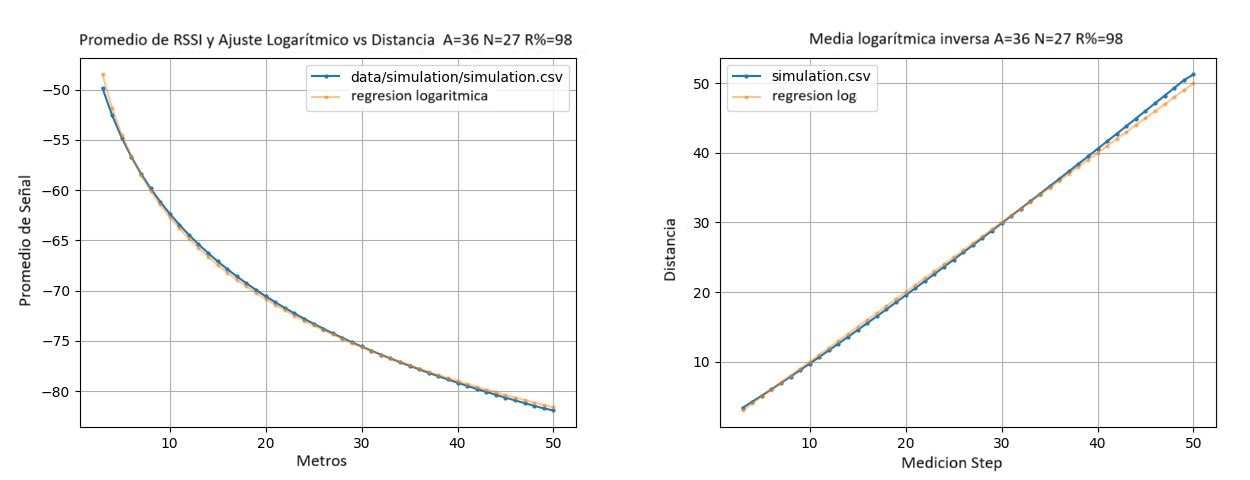
\includegraphics[width=0.99\textwidth]{Figuras/profiling/simulation/simulated-profiling-combo.jpg}
\captionsetup{margin=2cm}
\caption[ A la derecha, media de RSSI segregado por distancia de la medición vs regresión logarítmica, simulación usando NS3. A la izquierda, inversa al logaritmo de la distancia y distancia predicha en base a A y N calculados para la media del RSSI]{A la derecha, media de \acs{rssi} segregado por distancia de la medición vs. regresión logarítmica, simulación usando \acs{ns3}. A la izquierda, inversa al logaritmo de la distancia y distancia predicha en base a \textbf{A} y \textbf{N} calculados para la media del \acs{rssi}.}
\label{fig:profiling-result-sim}
\end{figure}
Se pudo observar una pequeña deriva entre la ubicación real y la predicha, esto se debe a que el \textit{fitting} de la curva simulada no es perfecto y tuvo un pequeño margen de error. Ese error depende de la distancia de la medición, ya que hay partes de la curva que se ajustan mejor que otras. En este caso, muy cerca del transmisor (menos de 1 metro) y al borde de la pérdida de transmisión (más de 45 metros) es donde más difieren, como se puede observar en la figura \ref{fig:profiling-result-sim}.
A pesar de ser un entorno simulado, estos resultados nos proporcionan una visión preliminar útil de cómo se comportaría nuestro sistema en la realidad, verificando que nuestros algoritmos funcionan y es posible ahora sí llevarlo a una prueba de campo. Los próximos pasos implicarán la realización de pruebas en entornos reales. Además, este experimento nos proporcionó valores de \textbf{N} y \textbf{A}, necesarios para nuestra fórmula de conversión de \acs{rssi} a distancia que se utilizarán luego en el experimento de multilateración simulado.
\section{Multilateración}
\subsection{Implementación}
Similar al experimento simulado de perfilado, se utilizó \acs{ns3}, esta vez con más nodos y haciendo un recorrido en dos dimensiones. Se utilizó el siguiente script para ejecutar la simulación \href{https://github.com/agusalex/ns3-rssi-trilateration/blob/main/src/2DTrilateration.cc}{\textbf{2DTrilateration.cc}}.
Además, para identificar inequívocamente una captura de un paquete emitido puntual, se utilizó \emph{millis} para segregar paquetes al momento de realizar la multilateración. De esta manera, si dos paquetes (dos entradas del archivo \textit{csv}) potencialmente distintos tienen el mismo valor en la columna \emph{millis}, se consideran el mismo paquete en un momento dado y se calculan en la misma ecuación de multilateración.
\begin{figure}[!htb]
\centering
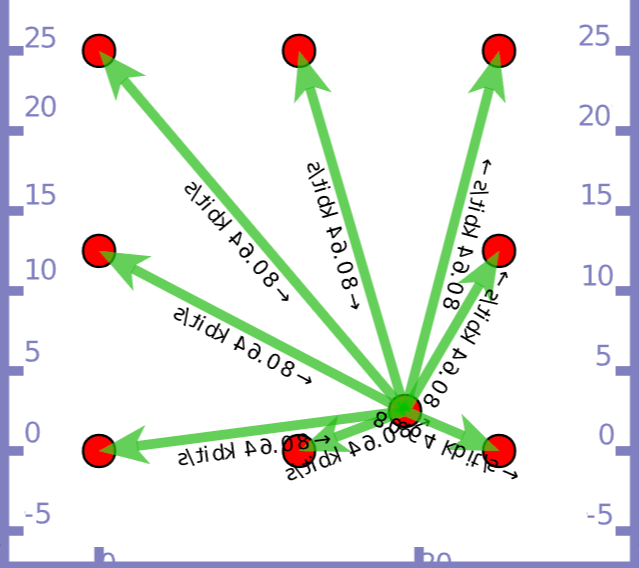
\includegraphics[width=0.5\textwidth]{Figuras/multilateration/simulated/multilateration-simulated-ns3.png}
\captionsetup{margin=2cm}
\caption[Visualización de la simulación de \acs{ns3}. El nodo objetivo realiza un recorrido mientras los otros ocho nodos Sniffer captan su señal.]{Visualización de la simulación de \acs{ns3}. El nodo objetivo realiza un recorrido mientras los otros ocho nodos \textit{Sniffer} captan su señal.}
\label{fig:simulated-ns3-mutilateration}
\end{figure}
\begin{table}[!htb]
\centering
\begin{tabular}{|c|c|c|c|c|c|c|c|}
\hline
millis & node & x & y & rssi & distance & target_x & target_y \\
\hline
9 & 2 & 12.5 & 0 & -63.5639 & 12.492 & 12.492 & 12.492 \\
9 & 4 & 25 & 12.5 & -63.5649 & 12.508 & 12.492 & 12.492 \\
9 & 5 & 0 & 12.5 & -63.5639 & 12.492 & 12.492 & 12.492 \\
9 & 7 & 12.5 & 25 & -63.5649 & 12.508 & 12.492 & 12.492 \\
9 & 1 & 0 & 0 & -68.0793 & 17.6664 & 12.492 & 12.492 \\
9 & 3 & 25 & 0 & -68.0799 & 17.6777 & 12.492 & 12.492 \\
9 & 6 & 0 & 25 & -68.0799 & 17.6777 & 12.492 & 12.492 \\
9 & 8 & 25 & 25 & -68.0804 & 17.689 & 12.492 & 12.492 \\
\hline
\end{tabular}
\caption{ Extracto de captura simulada que luego se usará como \textit{input} para multilateración. (Simulation.csv)}
\label{table:2}
\end{table}
El resultado de la ejecución es otro archivo \textit{csv} con las siguientes columnas: \textbf{millis}, \textbf{x}, \textbf{y}, \textbf{rssi}, \textbf{target\_x}, \textbf{target\_y}. \textbf{Millis} representa los milisegundos de la simulación, esto se usará luego para agrupar por ese criterio a la hora de hacer la multilateración. \textbf{X} e \textbf{Y} representan la ubicación del nodo que capturó el \textbf{rssi} de esa medición. Finalmente, \textbf{target\_x} y \textbf{target\_y} son la ubicación real del nodo \textbf{Objetivo} cuando la medición fue realizada, esto lo sabemos con certeza dado que el entorno es simulado.
Este archivo luego es procesado por nuestro algoritmo de multilateración, utilizando los valores de \textbf{A} y \textbf{N} hallados anteriormente para el perfilado simulado. Nuestro algoritmo de multilateración primero agrupa por paquetes que se hayan capturado al mismo momento, es decir, que los milisegundos (\textbf{Millis}) de la simulación sean los mismos. Luego solo se le aplicará multilateración y, de manera subsecuente, se agregarán al recorrido aquellos grupos de paquetes que al menos hayan sido capturados por 4 nodos o más. Esto se debe a que nuestro algoritmo de cuadrados mínimos necesita como mínimo al menos 4 nodos distintos para producir una predicción. Finalmente, se graficó el recorrido en 2d usando la biblioteca \textit{pyplot}.
\subsection{Experimento}
Inicialmente, se planteó un experimento con 4 nodos formando un cuadrado de 100x100 metros. Esto no produjo buenos resultados, ya que como el límite de recepción es alrededor de 50 metros, por momentos el nodo objetivo dejaba de estar al alcance de al menos 4 nodos y, entonces, la predicción fallaba. Esto se hacía evidente, produciendo recorridos que discrepaban enormemente del recorrido real. Al hacer más chico el cuadrado de 50x50 metros, la predicción se acerca mucho más a la realidad (Figura izquierda \ref{fig:ns3-multi-combined}). Finalmente, se diseñó un segundo recorrido de 25x25 metros, con 8 nodos (figura derecha \ref{fig:ns3-multi-combined}), mediante el cual se llegó al mejor resultado.
Usando \textbf{A = 36} y \textbf{N = 27} obtenidos durante el experimento de perfilado, se logró buena precisión a la hora de calcular el recorrido hecho por el nodo \textbf{Objetivo}.
\begin{figure}[!htb]
\centering
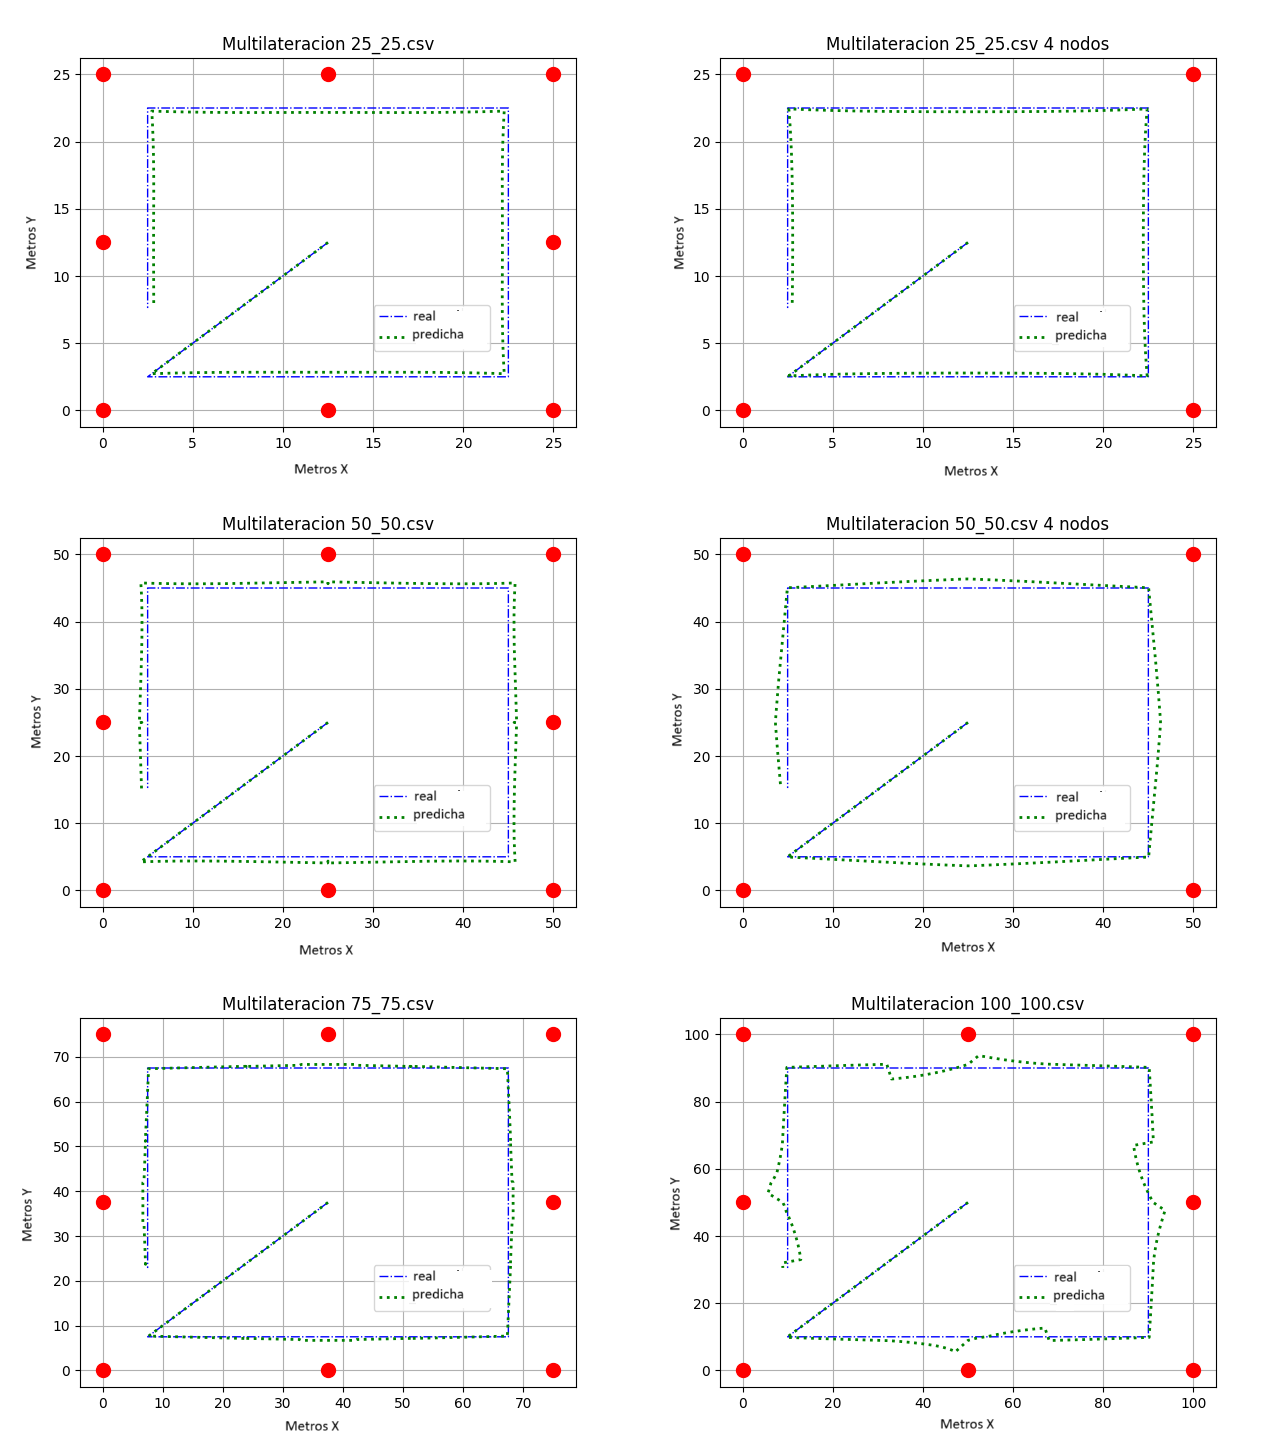
\includegraphics[width=0.99\textwidth]{Figuras/multilateration/simulated/many-sizes-and-node-count.png}
\captionsetup{margin=2cm}
\caption[Multilateración simulada]{Multilateración simulada. Se toman los datos de la simulación en \acs{ns3} más el \textbf{N} y \textbf{A} hallados y podemos conseguir ubicar a los nodos con los paquetes capturados. Se simularon distintos tamaños de grilla, desde 25x25 hasta 100x100. Cabe destacar que la precisión aumenta según la cantidad de nodos en el experimento y cuántos nodos reciben señal simultáneamente del objetivo. Esto último está relacionado al tamaño de grilla, ya que cuanto más lejos, menos nodos pueden recibir la señal.}
\label{fig:ns3-multi-combined}
\end{figure}
\section{Conclusión}
Se logró establecer un límite práctico en la cantidad mínima de nodos necesarios para determinar con precisión un recorrido durante una simulación, identificándose que con menos de cuatro nodos la predicción es inviable. Este requerimiento se explica por el uso de una ecuación tridimensional (involucrando las coordenadas \textit{x}, \textit{y} y el radio \textit{r}), a diferencia de los cálculos bidimensionales comúnmente usados cuando se realiza la técnica de trilateración, lo cual añade la precisión del radio a la medición pero exige un nodo adicional.
Este dato de precisión en la predicción (radio en metros de la predicción) es útil para poder descartar datos con mucho ruido. Adicionalmente, se observó que en escenarios con cuadrículas mayores a 50x50, la eficacia de la predicción disminuye progresivamente, atribuible a la reducción en el número de nodos receptores a medida que la distancia aumenta. Otro factor que incide en la pérdida de precisión es la creciente discrepancia entre las distancias predichas por el algoritmo durante la fase de perfilado y las distancias reales, particularmente al aproximarse a los 50 metros, punto en el que la capacidad de recepción del nodo transmisor se ve comprometida y la discrepancia aumenta, como se puede ver en la figura \ref{fig:profiling-result-sim}. Los experimentos de simulación, no obstante, arrojaron resultados prometedores, facilitando el desarrollo de técnicas y herramientas y permitiendo iterar rápidamente el proceso de desarrollo para encontrar soluciones en un entorno controlado. El perfilado proporcionó valores específicos para las variables \textbf{A} y \textbf{N}, cuya aplicación en experimentos de multilateración simulados confirmó la viabilidad del algoritmo. Esta fase de simulación culminó con buenos resultados, posibilitando avanzar hacia pruebas de campo por parte del equipo de investigación.